%%%%%%%%%%%%%%%%%%%%%%% file template.tex %%%%%%%%%%%%%%%%%%%%%%%%%
%
% This is a general template file for the LaTeX package SVJour3
% for Springer journals.          Springer Heidelberg 2010/09/16
%
% Copy it to a new file with a new name and use it as the basis
% for your article. Delete % signs as needed.
%
% This template includes a few options for different layouts and
% content for various journals. Please consult a previous issue of
% your journal as needed.
%
%%%%%%%%%%%%%%%%%%%%%%%%%%%%%%%%%%%%%%%%%%%%%%%%%%%%%%%%%%%%%%%%%%%
%
% First comes an example EPS file -- just ignore it and
% proceed on the \documentclass line
% your LaTeX will extract the file if required
\begin{filecontents*}{example.eps}
    %!PS-Adobe-3.0 EPSF-3.0
    %%BoundingBox: 19 19 221 221
    %%CreationDate: Mon Sep 29 1997
    %%Creator: programmed by hand (JK)
    %%EndComments
    gsave
    newpath
    20 20 moveto
    20 220 lineto
    220 220 lineto
    220 20 lineto
    closepath
    2 setlinewidth
    gsave
    .4 setgray fill
    grestore
    stroke
    grestore
\end{filecontents*}
%
\RequirePackage{fix-cm}
%
\documentclass{svjour3}                     % onecolumn (standard format)
%\documentclass[smallcondensed]{svjour3}     % onecolumn (ditto)
%\documentclass[smallextended]{svjour3}       % onecolumn (second format)
%\documentclass[twocolumn]{svjour3}          % twocolumn
%
\smartqed  % flush right qed marks, e.g. at end of proof
%
\usepackage{graphicx}
\usepackage{amssymb}
\usepackage{amsmath}
\usepackage[final]{pdfpages}
%
% \usepackage{mathptmx}      % use Times fonts if available on your TeX system
%
% insert here the call for the packages your document requires
%\usepackage{latexsym}
% etc.
%
% please place your own definitions here and don't use \def but
% \newcommand{}{}
%
% Insert the name of "your journal" with
% \journalname{myjournal}
%

\newcommand{\argmax}[1]{\underset{#1}{\operatorname{arg}\,\operatorname{max}}\;}

\begin{document}

    \title{Model-free Deep Reinforcement Learning -- Methods and Applications%\thanks{Grants or other notes
    %about the article that should go on the front page should be
    %placed here. General acknowledgments should be placed at the end of the article.}
    }
    \subtitle{Reinforcement Learning Seminar -- Winter Semester 2018/19}

    %\titlerunning{Short form of title}        % if too long for running head

    \author{Fabian Otto
    %    \and Second Author %etc.
    }

    %\authorrunning{Short form of author list} % if too long for running head

    \institute{Fabian Otto \at
    Technische Universit\"at Darmstadt, Computer Science Department\\
    %    Tel.: +123-45-678910\\
    %    Fax: +123-45-678910\\
    \email{fabian.otto@stud.tu-darmstadt.de}           %  \\
    %             \emph{Present address:} of F. Author  %  if needed
    %    \and
    %    S. Author \at
    %    second address
    }

    \date{Received: date / Accepted: date}
    % The correct dates will be entered by the editor


    \maketitle

    \begin{abstract}
        Insert your abstract here. Include keywords, PACS and mathematical
        subject classification numbers as needed.
        \keywords{Reinforcement Learning\and Neural Networks}
        % \PACS{PACS code1 \and PACS code2 \and more}
        % \subclass{MSC code1 \and MSC code2 \and more}
    \end{abstract}

    \section{Introduction \label{sec:intro}}
    \textit{Neural networks} (NN) have been used 
    
    \section{Background}
%    \paragraph{Markov Decision Process}
    A Markov Decision Process (MDP) is defined as a tuple $(\mathcal{S}, \mathcal{A}, \mathcal{T},\mathcal{R})$, where $\mathcal{S}$ is a finite set of states, $\mathcal{A}$ is a finite set of actions, $\mathcal{T}:\mathcal{S} \times \mathcal{A} \rightarrow \Pi(\mathcal{S})$ represents the state transition function, which returns a probability distribution over states and 
    $\mathcal{R}:\mathcal{S} \times \mathcal{A} \rightarrow \mathbb{R}$ returns the expected immediate reward for taking each action in each state. 
    This paper mainly considers the infinite horizon MDP, which tries to maximize the expected discounted cumulative reward:
    \[
    G_t = \mathbb{E} \left[ \sum_{\tau=t}^{\infty} \gamma^{\tau-t} \mathcal{R}(s_\tau,a_\tau)\middle|s_\tau,a_\tau \right]
	\]
    Here $\gamma \in \left[0,1\right)$ describes the discount factor, which trades of immediate and future rewards.\\
%    By choosing $\gamma=1$ and setting the horizon $k$ to an finite value, the optimization target of finite horizon MDP can be described.\\
    RL algorithms now aim to find a policy $\pi:\mathcal{S} \rightarrow \mathcal{A}$, which describes the optimal behavior to maximize the expected future reward from all states.
    Consequently, an action-value function, which returns the value of taking an action $a$ in state $s$, under the policy $\pi$ is defined as:
    \[
    Q_\pi(s,a) = \mathbb{E}\left[G_t|s_t =s,a_t=a,\pi\right] = \mathcal{R}(s,a) + \gamma \sum_{s\in\mathcal{S}}\mathcal{T}(s,a,s') \max_{a'}Q_\pi(s',a')
	\]
    In order to find the best policy, value-based methods are interested in finding the optimal action-value function $Q^*(s,a) =\max_\pi Q_\pi(s,a)$, which is equivalent to finding the optimal policy 
    \[
	\pi^*(s) = \argmax{a} \mathcal{R}(s,a) + \gamma \sum_{s\in\mathcal{S}}\mathcal{T}(s,a,s') \max_{a'}Q^*(s',a')
    \]
    Alternatively, the optimal value function $V^*(s) = \mathbb{E}\left[G_t|s_t=s, \pi\right] = \max_{a} Q^*(s,a)$ can be used, e.g. in combination with a model of the environment.\\
    In contrast to value-based methods, policy-based methods directly parameterize a policy $\pi(s;\theta)$. 
    One such method is REINFORCE \cite{Williams1992}, it updates the policy parameters $\theta$ in the direction $\nabla_\theta \mathbb{E}[G_t]\approx \nabla_\theta\log\pi(s_t;\theta)G_t$.
    In order to reduce variance and keeping the estimate unbiased, a baseline $b(s_t)$ is subtracted from the return $\nabla_\theta\log\pi(s;\theta)(G_t - b(s_t))$. 
    For this baseline, it is common to use an estimate of the value function $b(s_t)\approx V_\pi(s_t)$.
    By applying the policy gradient theorem, $G_t-b(s_t)$ can be seen as an estimate of the advantage function $A_\pi(s_t,a_t) = Q_\pi(s_t,a_t) - V_\pi(s_t)$.
    Combining parameterized policies and value function estimator results in \textit{actor-critic} (AC) methods. 
    


%    \section{Recent Approaches in Reinforcement Learning}
%    \label{sec:recent}
    \section{Algorithms \label{sec:algo}}
	This section provides an overview of the current deep RL landscape including improvements and current state-of-the-art. 
	Most algorithms can be either classified as on-policy or off-policy algorithms.
	On-policy algorithms estimate the value of policy while using it for control whereas off-policy algorithms, the generating policy, called \textit{behavior policy}, is not necessarily related to the \textit{target policy}, which is improved and evaluated.
	This allows to use a deterministic target policy, while still sampling all actions through the behavior policy. \cite[chapter 5]{Sutton2018}
	\begin{figure}[!htbp]
		\centering
		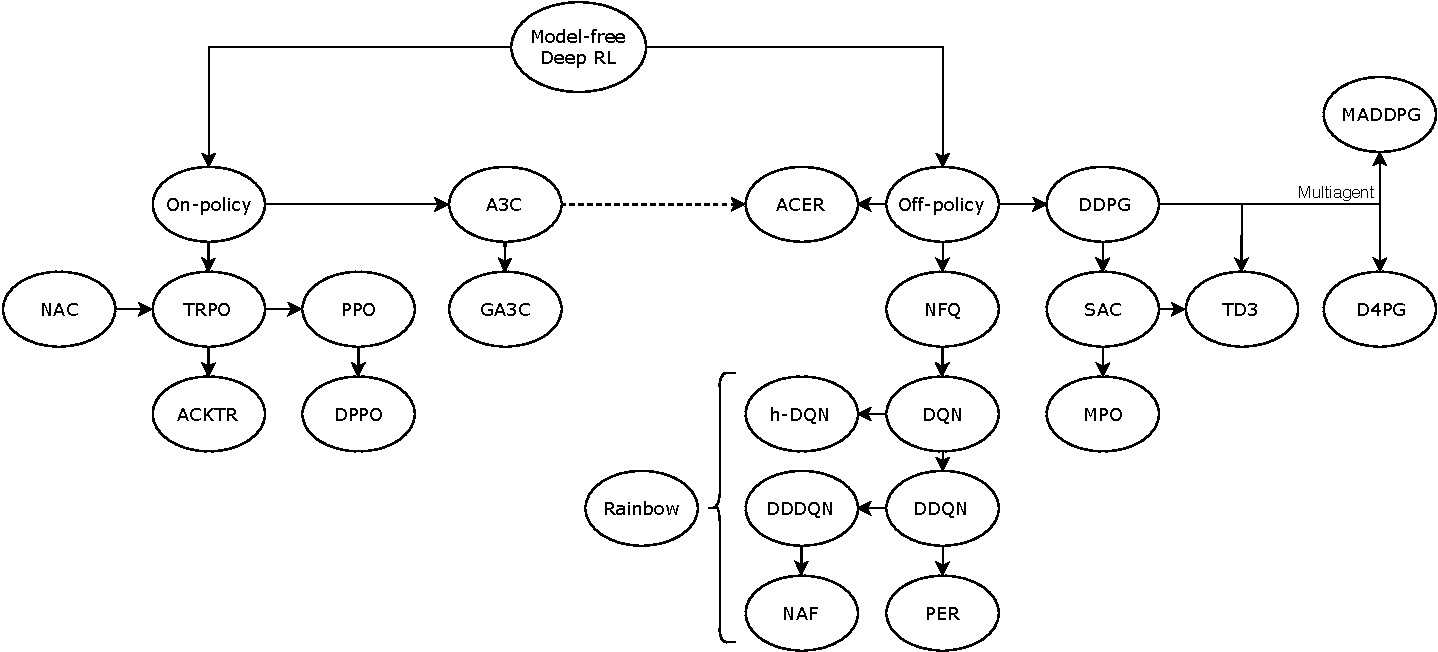
\includegraphics[angle=90]{images/tree.pdf}
		\caption{Test}
	\end{figure}

		
 	\subsection{Off-Policy \label{sec:off-policy}}
	One of the earlier off-policy algorithms, named \textit{neural fitted Q-iteration} (NFQ), was published by Riedmiller \cite{Riedmiller2005} in 2005. 
	NFQ works model-free based on vanilla Q-Learning \cite{Watkins1989} and approximates the action-value function with a multilayer-perceptron.
	Compared to other approaches at the time, NFQ allows to learn with a relatively good data efficiency.
	Further, batches from a replay memory \cite{Lin1992} are used in order to train the multilayer-perceptron with \textit{resilient backpropagation} (RPROP) \cite{Riedmiller1993}.
	Thereby, it is possible to dynamically add new samples to the replay memory during learning.
	Motivated by this idea as well as the success of TD-gammon \cite{Tesauro1994} the arguably biggest improvement in NN based RL -- \textit{Deep Q-Networks} (DQN) -- were introduced by Mnih, et al. \cite{Mnih2015}.   
	They built upon their prior results \cite{Mnih2013} on the Atari Arcade Environment \cite{Bellemare2013} which already achieved state-of-the-art performance for some of the games.
	DQNs introduce better scalability to larger data sets by replacing NFQ's RPROP with \textit{Stochastic Gradient Descent} (SGD) updates. 
	Further, they allow training end-to-end from the raw visual input utilizing \textit{convolutional neural networks} (CNN). 
	Benchmarks of the more recent DQN version \cite{Mnih2015} show an improved performance as well as a better generalization to more Atari games compared to initial work \cite{Mnih2013}.
	The performance improvement was mainly achieved by introducing a second target Q-network, which is only periodically updated and thereby reduces sample correlations. 
	However, van Hasselt, et al. \cite{VanHasselt2016} show that DQNs \cite{Mnih2015} are not sufficient to avoid overestimations of action-values under certain conditions. 
	This in itself is not harmful to the policy's performance, but if the overestimation is not uniform and not concentrated at the states of interest, it might affect the policy negatively. 
	To mitigate the risk of overestimation, they propose \textit{Double DQN} (DDQN).
	Double Q-Learning in general tries to decouple the selection and evaluation of actions by learning two action-value functions. 
	One determines the greedy policy and the other the value of this policy.  
	In order to reduce the computational cost, DDQN utilizes the already existing online Q-network for determining the greedy policy and the target Q-network for estimating its value. 
	Further, this allows to achieve better performance on most of the Atari games. 
	Decoupling is also done in a more extreme form with \textit{Dueling Double DQNs} (DDDQN) \cite{Wang2016}. 
	They introduce two separate function approximations, one for the state-value function and one for the state-dependent action-advantage function, in order to represent the action-value\footnote{Both estimators share parameters in the network's convolutional part and are trained together end-to-end.}.
	These estimators allow the dueling architecture to learn about the value of a state regardless of the action taken. 
	This is especially important when the action has no repercussions about the near future. 
	Combining DDQN with gradient clipping and \textit{prioritized experience replay} (PER) \cite{Schaul2015} shows that sampling rare experiences with a higher probability makes learning with replay memories more efficient \cite{Lin1992}. 
	However, sampling non-uniformly from the replay memory introduces a bias, that has to be corrected during the update step.\\
	All previous approaches are using environments, which do not have to deal with delayed and sparse feedback.
	In real world applications this is often not the case and algorithms still need the ability to learn.
	One key problem, which occurs during training, is insufficient exploration, thereby unstable policies. 
	Using intrinsically motivated agents, exploration can be achieved for the agent itself rather for an external goal. 
	This idea is implemented by \textit{hierarchical-DQN} (h-DQN) \cite{Kulkarni2016}, which is based on a hierarchy of two DQNs.
	A top level meta-controller is selecting a subgoal in order to optimize the extrinsic reward.
	The lower level controller maximizes an intrinsic reward by solving the subgoal.
	This allows h-DQN to achieve a significant better performance on the Atari game Montezuma's Revenge.
	A general comparison of different DQN version is presented by Hessel, et al. \cite{Hessel2018}\, they also introduce a new \
	As the above results show, Q-learning variations are successful for discrete action spaces, real world problems however often require continuous action spaces.
	Further, it is usually hard in real world applications to collect data from e.g. robots, and therefore dealing with high sample complexity.
	\textit{Normalized advantage functions} (NAF) \cite{Gu2016} approach both problems with a DQN based algorithm.
	Similar to DDDQN \cite{Wang2016}, the Q-network is represented by one state-value function output and one state-dependent action-advantage function.
	In order to reduce sample complexity, NAF incorporates imagination rollouts. 
	Those synthetic on-policy samples are created by utilizing a mixture of \textit{iterative LQG} (iLQG) \cite{Todorov2005} and on-policy trajectories for real world rollouts.
	Afterwards, the learned model for the states is used to generate replay memory entries. 
	This can be seen as a scalable variant of Dyna-Q \cite{Sutton1990}. 
	As a drawback, NAF failed to show improvements using iLQG compared to on-policy samples, however, iLQG might be desirable when damage avoidance is crucial. 
	Lillicrap, et al. \cite{Lillicrap2016} also adapt the underlying idea of DQN \cite{Mnih2015} and make it applicable to the continuous action domain. 
	However, they do not follow a value based learning and introduce \textit{Deep Deterministic Policy Gradients} (DDPG), a model-free AC algorithm with approximate Q-Learning based on deterministic policy gradients (DPG) \cite{Silver2014}.
	%		different class of algorithms, policy gradients methods.
	DQN's \cite{Mnih2015} architecture is improved by adding batch normalization layers \cite{Ioffe2015} to deal with different physical units in the observation space. 
	In order to stabilize policies, they adapt the idea of target networks from DQN \cite{Mnih2015} and use "soft" target updates for AC. 
	Albeit, this stability is, according to Haaranoja, et al. \cite{Haarnoja2018}, extremely difficult to achieve and further, DDPG is brittle to hyperparameter choices. 
	As consequence, Haaranoja, et al. present soft actor critic (SAC) \cite{Haarnoja2018}.
	They combine the AC approach from DDPG \cite{Lillicrap2016} with maximum entropy reinforcement learning, which enables exploration and stability. 
	Similarly to NAF \cite{Gu2016}, they also approach the problem of sample efficiency and gain significant improvements compared DDPG and several on-policy methods.
	In general they also found modeling the state-value function and the action-value function with two separate NNs improved the stability of SAC. 
	\textit{Twin delayed DDPG} (TD3) \cite{Fujimoto2018} was developed in parallel to SAC and continues to addresses the hyperparameter sensitivity, but further shows that overestimation of the action-value function is also a pressing issue for AC methods. 
	However, for the continuous actions space the approach of DDQN \cite{VanHasselt2016} is not easily applicable.
	Therefore, TD3 proposes three key improvements.
	A clipped variant of double Q-Learning \cite{VanHasselt2010} trains two separate Q-Networks in order to reduce the overestimation bias.
	Policy smoothing, similar to expected SARSA \cite{VanSeijen2009}, adds noise to the target action, which avoids exploiting Q-function errors and brings action-values of similar actions closer together.
	The most important improvement, however, are delayed updates, i.e. the policy network as well as the target networks are updated less frequently than the Q-network.
	This reduces the risk of optimizing the policy based on incorrect value estimates and hence the policy is less likely to diverge.	
	Building upon the idea of entropy reinforcement learning from SAC, Maximum a-Posteriori policy optimization (MPO) \cite{Abdolmaleki2018} transforms the RL problem in an inference problem, which allows them to utilize expectation maximization (EM) for training, while optimizing a relative-entropy objective.
	Combining DDPG with distributed actors, such as the on-policy \textit{asynchronous advantage actor critic} (A3C) \cite{Mnih2016}, and a distributional value estimate \cite{Bellemare2017} results in \textit{Distributional Distributed DDPG} (D4PG) \cite{Barth-Maron2018}.
	A3C also has an off-policy counterpart \textit{actor-critic with experience replay} (ACER) \cite{Wang2017}, which outperforms A3C by significant margin regarding performance and sample efficiency. 
	This is achieved by Retrace \cite{Munos2016} Q-value estimation, which reduces the bias of policy gradient estimates, whereas truncated importance weights help to reduce variance.
	Additionally, maintaining a running average of past policies forces the new policy to stay close to this average.
	This is similar to computing the \textit{Kullback-Leibler} (KL) \textit{trust region policy optimization} (TRPO), however it is computationally more efficient.
	The above algorithms used multiple agents to provide better exploration and faster convergence, however the goal was to find the optimal policy for one worker. 
	\textit{Multi-agent DDPG} (MADDPG) \cite{Lowe2017} on the other hand is interested in using multiple agents to collaborate and/or compete. 
%		However, this changes the problem setting of MADDPG to a Markov Game. 
	The decentralized actors are only trained with local information, which allows for easier inference, the centralized critics have access to all information during training. 
	In order to reduce variance due to interactions with other actors, policy ensembles are proposed. 
		
    \subsection{On-Policy}
    \label{sec:on-policy}
	Comparably important to DQN \cite{Mnih2015} in the off-policy setting is the introduction of \textit{asynchronous advantage actor critic} (A3C) \cite{Mnih2016} for the on-policy setting.
   	Besides A3C, Mnih, et al. also introduce asynchronous off-policy methods for Q-Learning and SARSA.
   	However, they show that A3C outperforms the proposed off-policy methods.
   	Multiple actor threads allow A3C to collect more experience in a larger space of the environment and incorporate it into one shared policy network.
   	Consequently, the stability and robustness of the training process is increased without incorporating a replay memory. 
	Further, less computational power is required to achieve better results compared to DQN \cite{Mnih2015}.\footnote{A3C only utilizes CPU computation compared to DQN's GPU computation for the Atari environments.}
	A3C was also combined with GPU computation \cite{Babaeizadeh2017}.
	Similar to SAC \cite{Haarnoja2018} entropy is included in objective function, however A3C utilizes it for regularization and not as constraint.
	Aside from the discrete Atari games, A3C was also tested for continuous action spaces and was able to learn reliable policies. 
    Following the concept of policy gradients, Schulman, et al. introduce trust region policy optimization (TRPO) \cite{Schulman2015}.
    TRPO can be seen as combination of minorization-maximization \cite{Hunter2004} and \textit{natural actor critic} (NAC) \cite{Peters2008a}
    They criticize that first order gradient methods are often overconfident and not accurate enough in curved areas, which results in losing already made learning progress. 
    Consequently, TRPO optimizes its policy by enforcing a trust region constraint. 
    The trust region constraint represents a pessimistic/lower bound on the performance of the policy and guarantees monotonic improvement locally around the current policy.	
    In order to be more computationally efficient, the natural policy gradient \cite{Kakade2001} is computed approximately with the \textit{Conjugate Gradient} (CG) algorithm.
    Further, due to the multiple approximations, before applying the update, a backtracking line search determines whether the update still satisfies the KL constraint or not. 
    One big drawback of TRPO in practice is its sample efficiency. 
    Theoretically, TRPO can be applied to any policy, but it is often not practical to use deep neural networks policies.
    This shortcoming is addressed by Proximal Policy Optimization (PPO) \cite{Schulman2017}.
    PPO keeps all monotonic improvement guarantees while using first order optimization by replacing the KL constraint with KL regularization.
    Addtionally, the importance sampling weights are  clipped, which results in a lower bound for the unclipped objective.
    PPO can also be combined with A3C's idea of distributed actors resulting into \textit{Distributed PPO} (DPPO) \cite{Heess2017}. 
    Besides PPO, \textit{actor-critic using kronecker-factored trust region} (ACKTR) \cite{Wu2017} also approaches TRPO's problem of sample complexity.
    ACKTR utilizes A3C's advantage function and approximates the natural gradient with \textit{kronecker-factored approximate curvature} (K-FAC) \cite{Grosse2016,Martens2015}, which offers a comparable cost to SGD. 
    By maintaining a running average of curvature information, K-FAC is able to reduce variance and achieve scalability, therefore ACKTR is more efficient in computing the inverse Fisher Information matrix. 
    Further, ACKTR is not only able to increase the performance and sample efficiency compared to TRPO but also compared to the synchronous version of A3C - A2C \cite{Mnih2016}. 
	
    \section{Applications in Games and Robotics}
    \label{sec:games}
    One of the earliest success stories of Deep RL was TD-gammon \cite{Tesauro1994} achieving master level performance in backgammon.
    TD-gammon was starting with zero prior knowledge and improved by solely playing against itself.
    However, consecutive experiments aiming to reproduce the success in backgammon for other games such as chess, Go, checkers failed.
    This was often attributed to the idea that state space exploration was helped by the stochasticity of the dice rolls \cite{Pollack1997}.
    Albeit these failures, DQN was motivated by this success a showed that it was not only able to outperform existing methods on most of the Atari games, but even surpass human-level performance. 
    RL algorithms following after DQN were able to improve the performance even further for all games (e.g. A3C) or specifically for poorly performing games, such as h-DQN on Montezuma's Revenge.
    Based on the idea of TD-gammon, AlphaGo \cite{Silver2016} combined self-play with CNNs, supervised learning and \textit{Monte Carlo Tree Search} (MCTS). 
    In its core AlphaGo is selecting moves by a novel MCTS, which is guided by learned a value function and policy.
    However, instead of directly training from scratch, value function and policy are pretrained on human expert moves and are afterwards improved by self-play.
    In 2016 AlphaGo showed significantly better performance compared to other programs and was able to achieve the first victories over professional players.
    AlphaGo Zero \cite{Silver2017a} eliminated the supervised learning aspect from AlphaGo and used no human data or guidance beyond the basic rules of the game.
    Additional improvements include an improved version of MCTS and the use of MCTS during training/self-play.
    AlphaGo Zero was able to defeat the strongest human players without a single loss and also beat AlphaGo considerably.
    AlphaZero \cite{Silver2017} generalizes AlphaGo Zero to the chess and shogi domain.
    As a consequence, AlphaZero has to take different outcomes, e.g. draws, into account, further it is not able to exploit symmetries such as in Go.
    One major criticism is the underlying computational power, e.g. training for AlphaZero was executed on 5,000 TPUs \cite{Jouppi2017}. 
    Therefore, it is questionable if the same algorithm performs equally well with less computational power. 
    
    \section{problems}
    convergence 
    hyperparams
    forgetting
    ???

    % BibTeX users please use one of
    %\bibliographystyle{spbasic}      % basic style, author-year citations
    \bibliographystyle{spmpsci}      % mathematics and physical sciences
    %\bibliographystyle{spphys}       % APS-like style for physics
    \bibliography{library2.bib}
    % name your BibTeX data base


\end{document}

